\documentclass{beamer}
\beamertemplatenavigationsymbolsempty
\usecolortheme{beaver}
\setbeamertemplate{blocks}[rounded=true, shadow=true]
\setbeamertemplate{footline}[page number]
%
\usepackage[utf8]{inputenc}
\usepackage[english,russian]{babel}
\usepackage{amssymb,amsfonts,amsmath,mathtext}
\usepackage{subfig}
\usepackage[all]{xy} % xy package for diagrams
\usepackage{array}
\usepackage{multicol}% many columns in slide
\usepackage{hyperref}% urls
\usepackage{tabularx}
\usepackage{hhline}%tables
% Your figures are here:
\graphicspath{ {fig/} {../figures/} }
\usepackage{amsmath}
\DeclareMathOperator*{\argmax}{arg\,max}
\DeclareMathOperator*{\argmin}{arg\,min}
\usepackage{algpseudocode}
\newcommand{\R}{\mathbb{R}}
\newcommand{\E}{\mathbb{E}}
\newcommand{\e}{\varepsilon}
\usepackage{algorithm}
\usepackage{algorithmic}
%\usepackage{arxiv}
%\documentclass[12pt]{article}
%\usepackage[cp1251]{inputenc}
%\usepackage[russian]{babel}
\usepackage[utf8]{inputenc}
\usepackage[english, russian]{babel}
\usepackage[T2A, T1]{fontenc}
\usepackage{url}
\usepackage{booktabs}
\usepackage{amsfonts}
\usepackage{nicefrac}
\usepackage{microtype}
\usepackage{lipsum}
\usepackage{comment}
\usepackage{graphicx}
\usepackage{natbib}
\usepackage{doi}
\usepackage{hyperref}
\usepackage{amssymb, amsmath, latexsym}
% \usepackage{fullpage}
\usepackage{algorithm}
\usepackage{algorithmic}
%\usepackage{algpseudocode}
\usepackage{tabularx}
\usepackage{paralist}
\usepackage{mathtools}
%\usepackage{tcolorbox}
\usepackage{xcolor}
\usepackage{amsmath}







%----------------------------------------------------------------------------------------------------------
\title[\hbox to 56mm]{Сходимость с оценкой вероятностей больших отклонений для задач выпуклой оптимизации и седловых задач в условиях повышенной гладкости}

\author[Д.\,Н. Рубцов]{Денис Николаевич Рубцов}
\institute{Московский физико-технический институт}
\date{\footnotesize
\par\smallskip\emph{Научный руководитель:} д.ф.-м.н. А.\,В.~Гасников

\par\bigskip\small 2024}
%----------------------------------------------------------------------------------------------------------
\begin{document}
%----------------------------------------------------------------------------------------------------------
\begin{frame}
\thispagestyle{empty}
\maketitle
\end{frame}
%-----------------------------------------------------------------------------------------------------
\begin{frame}{Цель исследования}
     \begin{block}{Цели}
     \begin{itemize}
         \item разработать быстрые алгоритмы для решения задач выпуклой оптимизации и седловыз задач с высокой вероятностью сходимости
         \item разработать ускоренные версии алгоритмов в условиях повышенной гладкости функций
     \end{itemize}
     \end{block}

 \end{frame}
%-----------------------------------------

%--------------------------------------------
 \begin{frame}{Тяжелые хвосты распределения шума стохастического градиента}

\begin{figure}
\caption*{ Гистограмма распределения шума стох.градиента для датасета "australian" из библиотеки LIBSVM. Красная линия аппроксимирует гистограмму функцией плотности нормального распределения. }
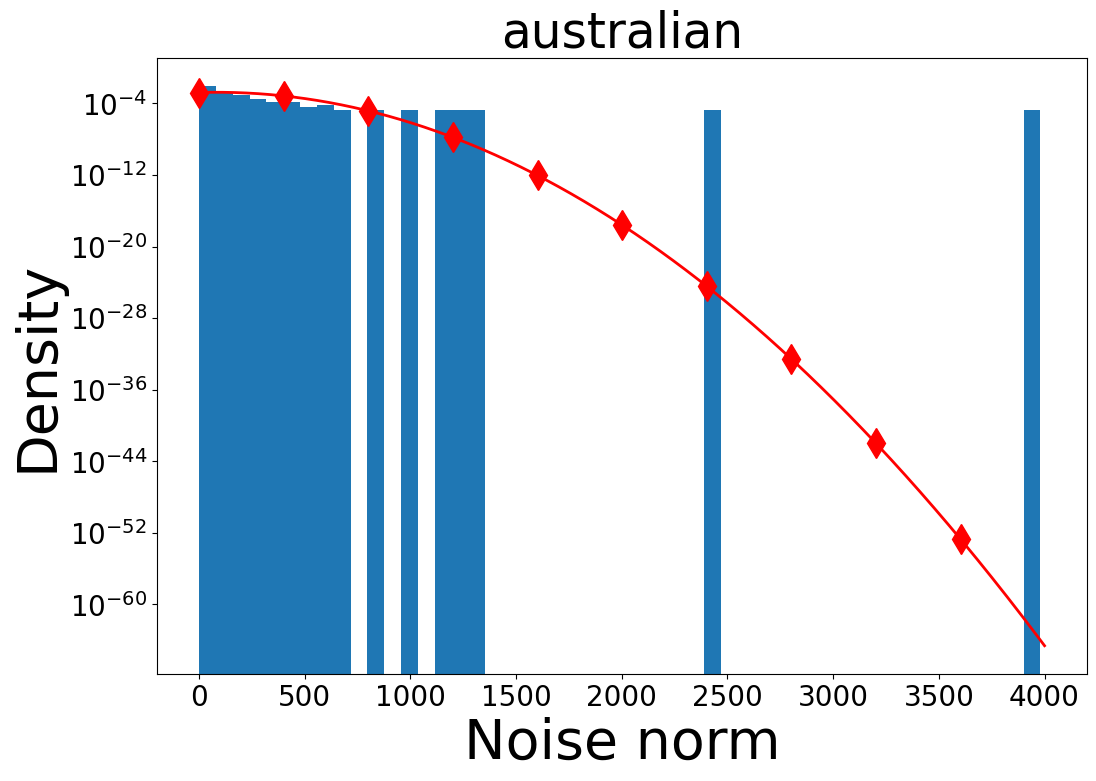
\includegraphics[width=0.7\textwidth]{australian_heavy_tails.png}
\end{figure}
\end{frame}

%---------------------

 \begin{frame}{Постановка задачи}
Задача стохастической оптимизации \[\min_{x \in \mathbb{R}^d} f(x) := \E{f(x, \xi)}, \ \xi \sim \mathcal{P}\]

Как правило, результатом стохастических градиентных методов является точка $x_{\e}$ такая, что 
\[\E{f(x_{\e})} - \min f \le \e\]

Мы рассматриваем алгоритмы, результатом которых являются точки $x_{\e, p}$, удовлетворяющие условию
\[\mathds{P} \{f(x_{\e, p})-\min f \le \e\} \ge 1 - p\]
где <<уровень уверенности>> $1 - p$ может быть достаточно большим


\end{frame}
%------------------------
 \begin{frame}{Постановка задачи}
Если решить задачу $\E{f(x_{\e})} - \min f \le p\e$, то желаемое неравенство $\mathds{P} \{f(x_{\e, p})-\min f \le \e\} \ge 1 - p$ следует автоматически по неравенству Маркова. 
\\
Сложность решения задачи сходимости по матожиданию, обычно, порядка $\mathcal{O} (\frac{1}{\e})$. Тогда сложность наивного решения задачи сходимости с высокой вероятностью $\mathcal{O} (\frac{1}{p\e})$. Хочется уменьшить множитель $\frac{1}{p}$ до $\ln(\frac{1}{p})$


\end{frame}
%-------------------------------
\begin{frame}{Robust distance estimation (RDE)}

Обозначим за $\mathcal{D}(\e)$  - оракул, возвращающий точку $x$: $\E{f(x)} - \min f \le \frac{\e}{3}$, т.е. $\mathds{P}[||x-x^*|| \le \e] \ge \frac23$. Можно сделать $m$ вызовов этого оракула $x_1, ..., x_m$ и выбрать среди полученных точек такую $x_{i^*}$, вокруг которой класстеризуются остальные точки.

\begin{columns}[c]
\column{0.4\textwidth}
\begin{theorem}
Точка $x_{i^*}$, возвращаемая алгоритмом RDE удовлетворяет условию
\[\mathds{P} (||x_{i^*} - x^*|| \le 3 \e) \ge 1 - e^{-\frac{m}{18}}\]
\end{theorem}
\column{0.6\textwidth}
\begin{figure}
\caption{Идея метода RDE}
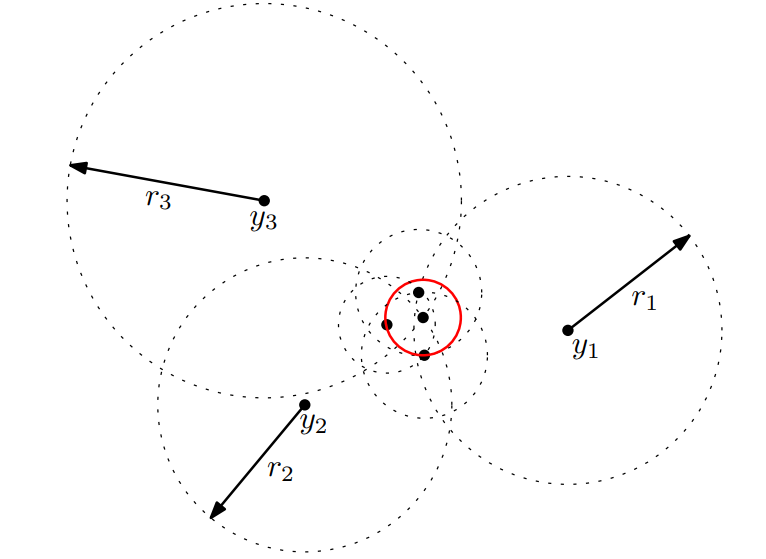
\includegraphics[width=\textwidth]{RDE.png}
\end{figure}
\end{columns}

\end{frame}
%------------------------
 \begin{frame}{Применение RDE для обеспечения сходимости с высокой вероятностью: описание подхода}

\[\frac{\mu}{2} ||x- x^*||^2 \le f(x) - f(x^*) \le \frac{L}{2} ||x - x^*||^2\]

Пусть мы имеем точки $x_i$ ($i = 1, ..., m$) такие, что 
\[\E{f(x_i)} - \min f \le \frac{\e}{3} \xRightarrow{\text{неравенство Маркова}}\]

\[\mathds{P} (f(x_i) - f^* \le \e ) \ge \frac{2}{3}\xLongrightarrow{\text{сильная выпуклость}}\]

\[\mathds{P} (||x_i - x^*|| < \sqrt{\frac{2 \e}{\mu}} =: \delta) \ge \frac{2}{3}\xLongrightarrow{\text{RDE}}\]

\[\mathds{P}(||x_{i^*} - x^*|| < 3 \delta) \ge 1 - e^{-\frac{m}{18}}\xLongrightarrow{\text{гладкость}}\]

\[\mathds{P}(f(x_{i^*}) - f^* \le  9 \frac{L}{\mu}\e) \ge 1 - e^{-\frac{m}{18}}\] 


\end{frame}
%------------------------
 \begin{frame}{Применение RDE для обеспечения сходимости с высокой вероятностью: проблема}

\[\E{f(x_i)} - \min f \le \frac{\e}{3} \xRightarrow{\text{...}}\]

\[\mathds{P}(f(x_{i^*}) - f^* \le  9 \frac{L}{\mu}\e) \ge 1 - e^{-\frac{m}{18}}\] 
Таким образом, генерируя точки алгоритмом, дающим гарантии сходимости с точностью $\e$ по матожиданию, но не с высокой вероятностью, мы предъявили алгоритм, дающий гарантию сходимости с высокой вероятностью, но лишь с $\kappa \e$-точностью, где число обусловленности $\kappa = \frac{L}{\mu} \gg 1$ может быть достаточно большим. 


\end{frame}
%-------------------------------
 \begin{frame}{Проксимальный метод $proxBoost$}

Зафиксируем возрастающую последовательность $\lambda_0, ..., \lambda_T$ и последовательность точек $x_0, ..., x_T$. На каждой итерации $i = 0, ..., T$ будем решать задачу минимизации не функции $f$, а функции $f^i$
\[f^i(x):=f(x) + \frac{\lambda_i}{2}||x - x_i||^2\]
\[\bar{x}_{i + 1} := \argmin_x f^i (x)\]


Число обусловленности новых функций можно сделать значительно меньше $\kappa_i = \frac{L + \lambda_i}{\mu + \lambda_i} = (\lambda_i = \mu \cdot 2^i) = \frac{L + \mu \cdot 2^i}{\mu + \mu \cdot 2^i} = \mathcal{O}(1)$ при $i > \log{\frac{L}{\mu}}$

При этом решение новых задач будет приближенным решением основных задач 
\[f(x_{j + 1}) - f^* \le (f^j(x_{j + 1}) - f^j(\bar{x}_{j + 1})) + \sum_{i = 0}^{j}\frac{\lambda_j}{2}||\bar{x}_i - x_i||^2.\]

\end{frame}
%-------------------------------
\begin{frame}{Сложность алгоритма proxBoost}
\begin{theorem}
    Пусть имеется оракул $\mathcal{M}(f, \e)$, возвращающий точку $x_{\e}$ такую, что $\mathds{P} (f(x_{\e})-\min f \le \e) \ge \frac{2}{3}$. Стоимость вызова такого оракула обозначим за $\mathcal{C}_{\mathcal{M}}(f, \e)$. Тогда для $\mu$-сильно выпуклых $L$-гладких функций алгоритм, решающий задачу $\mathds{P} \{f(x_{\e, p})-\min f \le \e\} \ge 1 - p$ требует \[\log({\frac{\log{\kappa}}{p}})\log{\kappa}\cdot \mathcal{C}_{\mathcal{M}}(f, \frac{\e}{\log{\kappa}}).\] 
\end{theorem}


\end{frame}

%-----------------------------------------------------------------------------------------------------
\begin{frame}{Метод регуляризации для решения не сильно выпуклых задач}
\begin{theorem}
    Пусть функция $f(x)$ выпукла. Будем решать задачу минимизации функции \[f^{\mu}(x) = f(x) + \frac{\mu}{2} ||x - x_0||^2,\] где $\mu \sim \frac{\e}{R^2}, R = ||x^* - x_0||$.

    Пусть мы нашли точку $x$ такую, что
    \[f^{\mu}(x) - \min f^{\mu} < \frac{\e}{2}\]
    Тогда 
    \[f(x) - \min f < \e\]
\end{theorem}
\end{frame}

%-----------------------------------------------------------------------------------------------------
\begin{frame}{Сложность алгоритма proxBoost в выпуклом случае}
\begin{theorem}
    Обобщение алгоритма $proxBoost$ для \textbf{выпуклых} $L$-гладких функций алгоритм, решающего задачу $\mathds{P} \{f(x_{\e, p})-\min f \le \e\} \ge 1 - p$ требует \[\log({\frac{\log{\frac{LR^2}{\e}}}{p}})\log{\frac{LR^2}{\e}}\cdot \mathcal{C}_{\mathcal{M}}(f, \frac{\e}{\log{\frac{LR^2}{\e}}}).\] 
\end{theorem}


\end{frame}
%-----------------------------------------------------------------------------------------------------

%-----------------------------------------------------------------------------------------------------




%-----------------------------------


%----------------------------------------------------------------------------------------------------------

%----------------------------------------------------------------------------------------------------------

%----------------------------------------------------------------------------------------------------------
\begin{frame}{Заключение}
     \begin{block}{Результаты}
     \begin{itemize}
         \item[-] алгоритм proxBoost для решения задач стохастической оптимизации сильно выпуклых функций обобщен для не сильно выпуклых функций

     \end{itemize}
     \end{block}
     \begin{block}{Планы}
     \begin{itemize}
         \item[-] проведение численных экспериментов сходимости предложенных методов
         \item[-] разработка аналогичных алгоритмов для седловых задач
         \item[-] использование повышенной гладкости функций для ускорения алгоритмов
     \end{itemize}
     \end{block}
 \end{frame}
%----------------------------------------------------------------------------------------------------------
%-----------------------------------



\end{document} 
